\begin{frame}{Nonnegative Rank}
\begin{defn}[Nonnegative rank]
Given $X \in \real_+^{p\times n}$, the nonnegative rank of \(X\), denoted $\rank_+(X)$ is the minimum $r$ such that there exist $W \in \real_+^{p\times r}, H \in \real_+^{r\times n}$ with $X = WH$.
\end{defn}
\centering
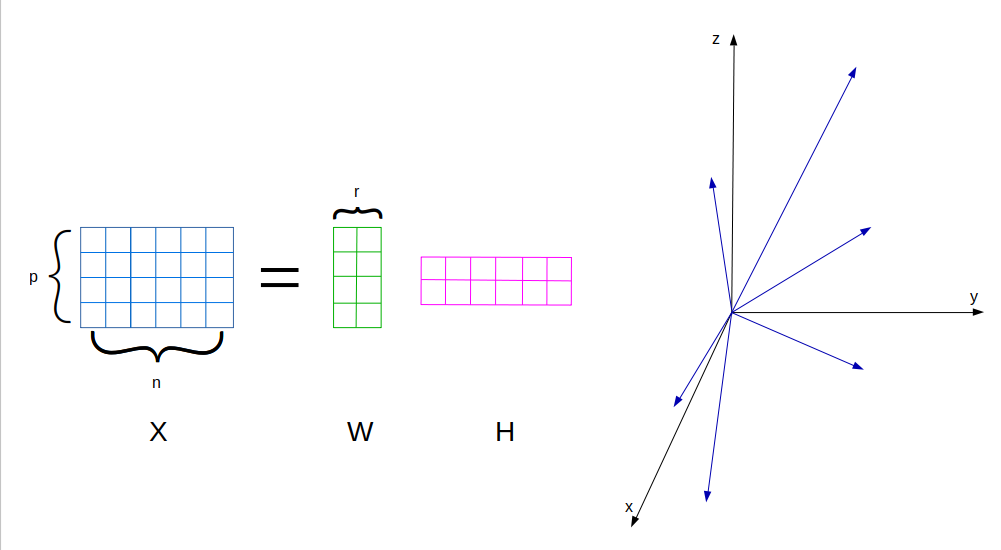
\includegraphics[scale=0.28]{../images/NMFvect.png}
\end{frame}
\begin{comment}
\begin{frame}{Computational Geometry : Nested polytopes problem}
\begin{figure}
\centering
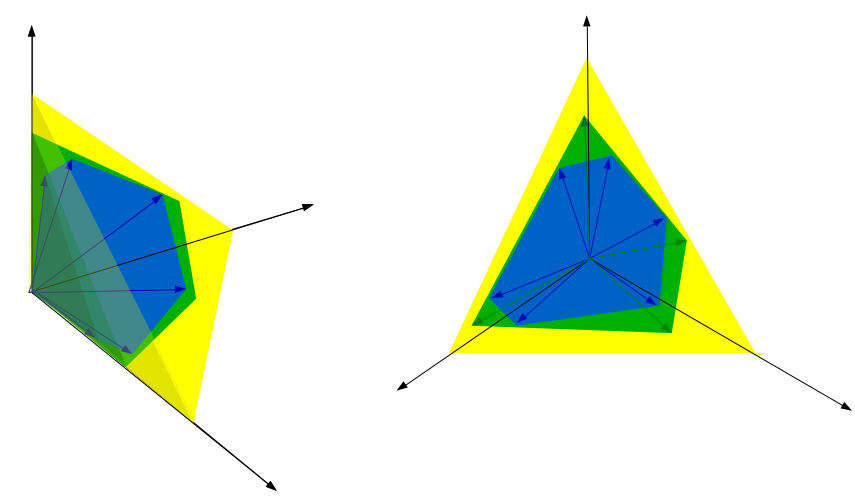
\includegraphics[scale=0.35]{../images/polytopeGeo.png}
\caption{\footnotesize Finding a polytope with minimum nb of vertices nested between 2 polytopes}
\end{figure}
\end{frame}
\end{comment}
\begin{frame}{Graph Theory: Bipartite Dimension}
Let $G(X) = (V_1 \cup V_2, E)$ be the bipartite graph induced by $X$ (i.e. $(i,j)\in E \iff X(i, j) \neq 0$).
\begin{defn}[Biclique and bipartite dimension]
\begin{itemize}
\item A \emph{biclique} (or \emph{complete bipartite graph}) is a bipartite graph such that every vertex in $V_1$ is connected to every vertex in $V_2$. 
\item The \emph{bipartite dimension} (or \emph{minimum biclique cover}) $\bc\big(G(X)\big)$ is the minimum number of bicliques needed to cover all edges in $E$.
\end{itemize} 
\end{defn}

\end{frame}

\begin{frame}{Graph Theory: Bipartite Dimension}

\begin{figure}
\centering
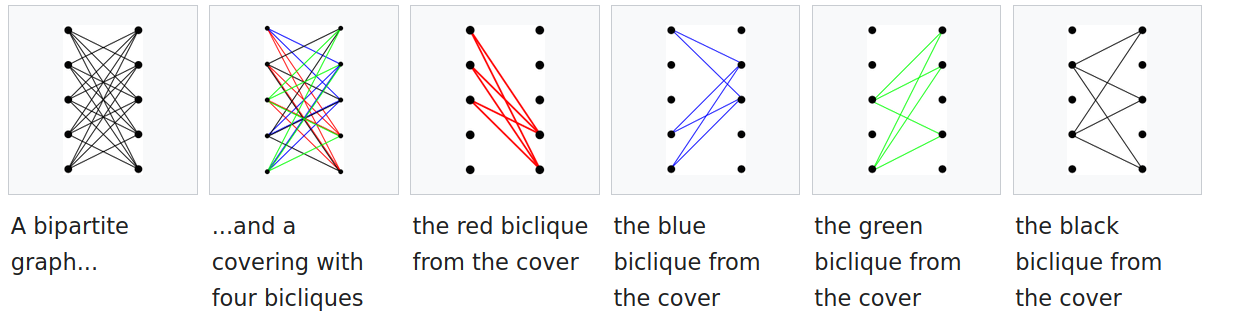
\includegraphics[scale=0.2]{../images/biclique.png}
\caption{Example of a biclique edge cover}
\end{figure}
\begin{thm}[Rectangle covering bound]
\[
\bc\big(G(X)\big)\leqslant \rank_+(X).
\]
\end{thm}
\end{frame}
\begin{comment}
\begin{frame}{Communication complexity}
\begin{center}

\includegraphics[scale=0.2]{../images/communication.png}
\end{center}
\small
Alice and Bob want to compute :
\[f:\{0,1\}^m \times \{0,1\}^n \rightarrow \{0,1\} : (x,y) \rightarrow f(x,y)
\]
While minimizing the nb of bits exchanged (i.e. communication complexity (CC)).


\textbf{Nondeterministic comm. complex. of $f$ (NCC)}: CC of $f$ with oracle/ message before starting the communication.


The communication matrix $X \in \{0,1\}^{2^n\times 2^m}$ is equal to the function $f$ for all possible combinations of inputs.

\begin{thm}[Yannakis]
\[\text{NCC of } f \leq \log_2(\text{rank}_+(X))
\]
\end{thm}
\end{frame}
\end{comment}
\begin{frame}{Linear Optimization: Extended Formulation}
\[
\begin{array}{l@{\quad}rcl}
\max \quad c^\top x&&& \\
\textnormal{s.t.} & Ax & \leqslant & b\\
& x \in \real^n & \geqslant & 0
\end{array}
\tag{LP}
\]
\begin{defn}[Extended formulation]
The \emph{extended formulation} of a polytope $P$ is a higher dimensional polytope $Q$ and a linear projection $\pi$ such that $\pi(Q) = P$.
\end{defn}
In (LP), an extended formulation of the polytope $P \subset \real^n$ defined by the constraints $Ax\leqslant b$, is a polytope $Q\subset \real^{n+r}$ defined by $Cx+Dy \leqslant d$ with $y\in \real^r$, such that $\pi(Q) = P$.

\end{frame}

\begin{frame}{Linear Optimization: Extended Formulation}
We define the \emph{slack matrix} $X(i,j) = b_i-A_iv_j$, with $v_j$ the $j$-th vertex of $P$ and $\{x\in \real^n \mid b_i-A_ix\geqslant 0\}$ its $i$-th facet.

\(X(i, j)\) measures the slack of the $i$-th inequality for the $j$-th vertex.

\begin{thm}[Yannakis]
The \emph{minimum size} of an extended formulation $Q$ of $P$ is equal to $\rank_+(X)$.
\end{thm}

When $P$ has exponentially many facets, finding extended formulations allows to solve (LP) in polynomial time.
\end{frame}